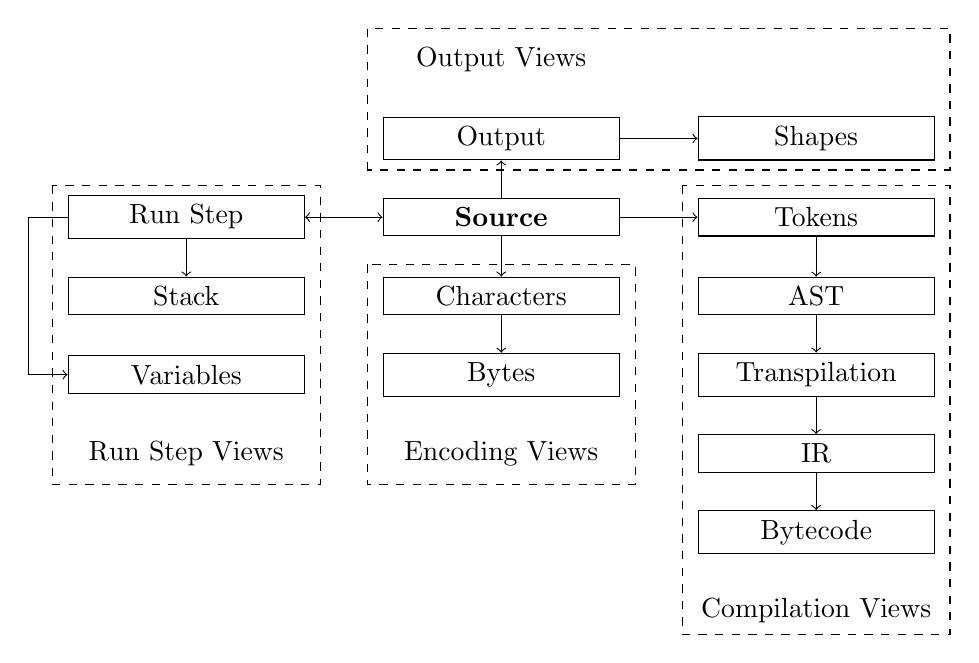
\begin{tikzpicture}

\node [draw, rectangle, minimum width=3cm] (source) at (0, 0) {\textbf{Source}};
\node [draw, rectangle, minimum width=3cm] (output) at (0, 1) {Output};
\node [draw, rectangle, minimum width=3cm] (tokens) at (4, 0) {Tokens};
\node [draw, rectangle, minimum width=3cm] (ast) at (4, -1) {\ac{AST}};
\node [draw, rectangle, minimum width=3cm] (transpilation) at (4, -2) {Transpilation};
\node [draw, rectangle, minimum width=3cm] (ir) at (4, -3) {\ac{IR}};
\node [draw, rectangle, minimum width=3cm] (bytecode) at (4, -4) {Bytecode};

\node [draw, rectangle, minimum width=3cm] (runstep) at (-4, 0) {Run Step};
\node [draw, rectangle, minimum width=3cm] (stack) at (-4, -1) {Stack};
\node [draw, rectangle, minimum width=3cm] (variables) at (-4, -2) {Variables};

\node [draw, rectangle, minimum width=3cm] (characters) at (0, -1) {Characters};
\node [draw, rectangle, minimum width=3cm] (bytes) at (0, -2) {Bytes};

\node [draw, rectangle, minimum width=3cm] (shapes) at (4, 1) {Shapes};

\draw [->] (source) -- (output);
\draw [->] (output) -- (shapes);
\draw [->] (source) -- (tokens);
\draw [->] (tokens) -- (ast);
\draw [->] (ast) -- (transpilation);
\draw [->] (transpilation) -- (ir);
\draw [->] (ir) -- (bytecode);
\draw [<->] (runstep) -- (source);
\draw [->] (runstep) -- (stack);
\draw [->] (runstep.west) -- +(-0.5, 0) |- (variables);
\draw [->] (source) -- (characters);
\draw [->] (characters) -- (bytes);

\draw [dashed] (-1.7, 0.6) rectangle (5.7, 2.4);
\node at (0, 2) {Output Views};
\draw [dashed] (2.3, 0.4) rectangle (5.7, -5.3);
\node at (4, -5) {Compilation Views};
\draw [dashed] (-1.7, -0.6) rectangle (1.7, -3.4);
\node at (0, -3) {Encoding Views};
\draw [dashed] (-5.7, 0.4) rectangle (-2.3, -3.4);
\node at (-4, -3) {Run Step Views};

\end{tikzpicture}
